\chapter{Conclusions}

In this chapter we summarize the foundings of analysed experiments from \textbf{Experimental Results} chapter and of numericalal experiments ftom the \textbf{Simulation} chapter.

\section{Experimental conclusions}

We investigated systematic high-Stokes flows of Helium-II at a range of temperatures $T \in \langle 1.35 \unit{K}, 2.17 \unit{K} \rangle$ generated by several types of oscillators - \textit{vibrating wire, torsionally oscillating disc and tuning
fork}. All of them were kept in high-frequency limit to ensure the Stokes number to be St$\gg 1$.

Within the area of \underline{low peak velocities}, we showed the normal component behaving laminar ($C_D^{\, n} \propto \text{Dn}^{-1}$) and superfluid component remaining potential (or stationary in case of torsional disc).\\
When we consider only a \underline{negligible amount} of remnant quantized vortices attached to the oscillator body, the normal and superfluid components have independent velocity fields, so the measured drags can be analysed separately as well. In this limit we treat the normal component as a classical viscous fluid, resulting naturally in inverse scaling of measured normal drag coefficient with the Donnelly number: $C_D^{\, n} \propto \text{Dn}^{-1}$.\\
Assuming that superfluid component doesn't contribute to the drag, the universal scaling holds until a critical velocity $U_C$ for a given oscillator geometry is reached. Or, generalising it for all oscillator modes $\{\omega_i\}$, until a \underline{critical dimensionless velocity} $\hat{U}_C = U_{C_i} / \sqrt{\varkappa \omega_i}$ is reached.

In general, we distinguish between \underline{4 types} of hydrodynamical states of Helium-II. We label the instabilities formed due to normal component as "CT" (classical turbulence) and due to superfluid component as "QT" (quantum turbulence):

\begin{itemize}
	\item \underline{No CT nor QT present:} laminar regime as described above, working universal scaling on normal component, superfluid component is potential or not moving at all, observed with all used oscillators ($\text{Dn} \lesssim 1$ for vibrating wire, $\text{Dn} \lesssim 5$ for oscillating disc and $\text{Dn} \lesssim 10$ for both oscillation modes of tuning fork).

	\item \underline{CT present without QT:} normal component expected to start exhibiting a classical non-linear behaviour after reaching critical value of Donnelly number $\text{Dn}_C$ (thus universal scaling still holds), superfluid component expected to remain potential or motionless, observed only with tuning fork at both oscillation modes for temperatures higher than $T > 1.6\unit{K}$ with low Donnelly numbers between $10 \lesssim \text{Dn} \lesssim 100$.

	\item \underline{QT present without CT:} occurs if critical velocity $U_C$ given by Donnelly-Glaberson instability (reconnection of remnant vortices) is achieved sooner than the critical Donnelly number $\text{Dn}_C$. Generally it is hard to prove whether such situation occured since the CT is usually triggerred almost immediately due to thw mutual friction.

	\item \underline{Both CT and QT present:} both normal and superfluid components are expected to contribute to the drag, occuring when both critical velocity $U_C$ and Donnelly number $\text{Dn}_C$ are reached (or triggerred), observed with all used oscillators.
\end{itemize}

To summarize, Donnelly-Glaberson instability (launching QT) occurs upon reaching a \textbf{critical dimensionless velocity} $\hat{U}_C$, while the instability in the normal component is governed  upon reaching a \textbf{critical Donnelly number} $\text{Dn}_C$. All of the phase states were observed during experiments on oscillating bodies as described in previous chapters.

We summarize all oscillators, once again in the \textit{flow phase diagram} in \textbf{Figure \ref{flow_phase_diagram}}:

\begin{figure}[h]
	\centering
	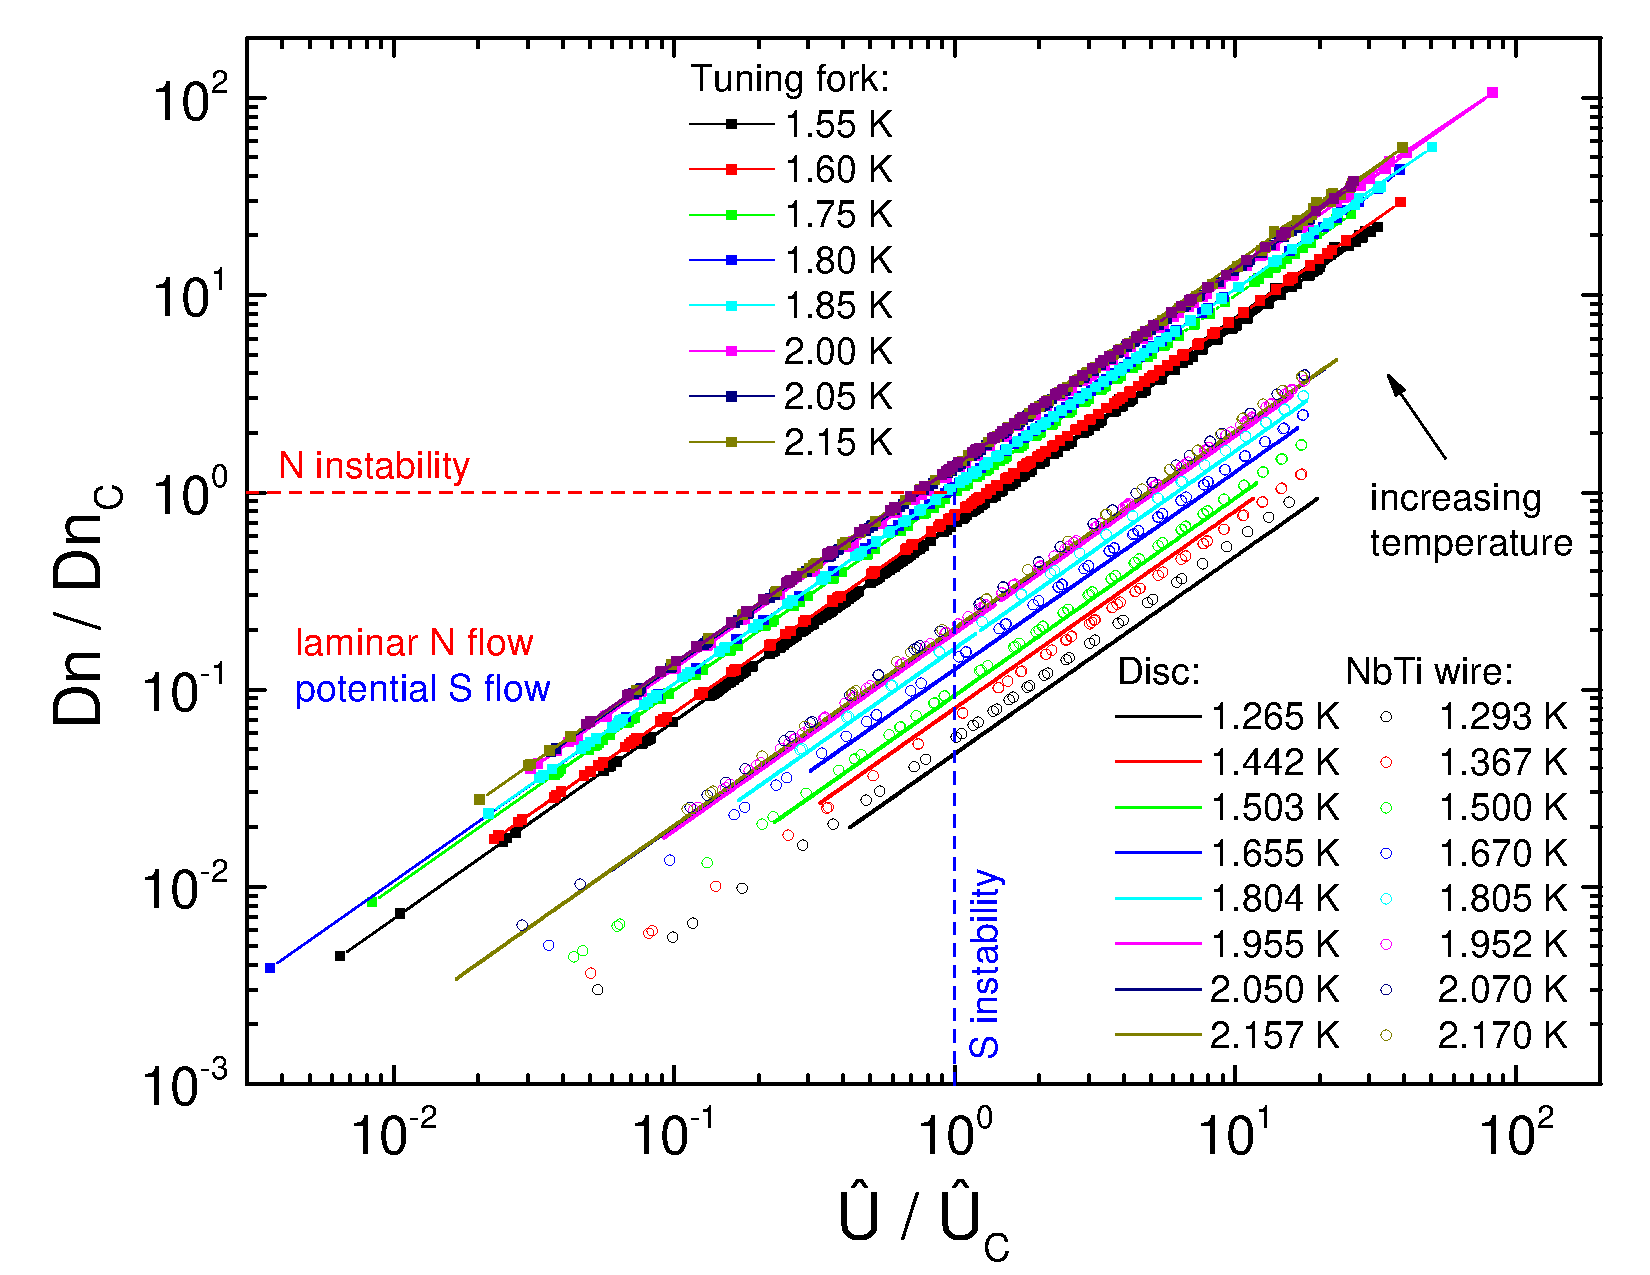
\includegraphics[width=0.8\textwidth]{graphics/results/flow_phase_diagram}
	\caption{Plot of Donnelly numbers against dimensionless velocities for three oscillators - vibrating wire, oscillating disc and tuning fork - submerged in Helium-II.\\
	\underline{Dashed lines} mark the estimated areas of transition from laminar/potential regimes to the non-linear ones, both for normal and superfluid components. The data used as a tuning fork is sourced from a different experiment, exhibiting the same behaviour.}
	\label{flow_phase_diagram}
\end{figure}

Vibrating wire and oscillating disc reach QT \underline{as the first transition}. From that, it is questionable when the CT was exactly triggerred since the exact bahaviour of QT evolution with oscillation velocity is not yet known. However, the tuning fork was the only oscillator that \underline{encountered the CT earlier than QT} for a certain tmeperatures $T \gtrsim 1.6\unit{K}$.\\
Which instability occurs as the first depedens both on geometry of the oscillator and temperature. Nevertheless, phase flow diagram proved itself as an useful visualisation for such purpose.

Additionally, we presented a formalism allowing the comparison between measurements in \underline{hydrodynamical} and \underline{non-newtonian} (thus ballistic) regimes of Helium-II. We have confirmed the universal scaling concept suggested for laminar flows in high-frequency limit, using the scaling function $f(\text{Wi})$.\\
However, the transitional flow regime ($\text{Wi} \sim 0.1$) reamins an open challenge to the theoretical and experimental investigation.


\section{Simulation conclusions}

We proposed an effective numerical method to compute the time evolution of vortex ring in superfluid He-II. All numerics is implemented in Python 3 and publicly uploaded on \href{https://github.com/KuboBahyl/superfluid}{GitHub} repository.\\
Performance of vortex filament model was improved by neglegcting the Biot-Savart integral, showing that the percentual errors are small, and updating the LIA calculation instead. Simulation well replicates the physical processes and performs with sufficient stability when using testing vortex ring of radius $R \in \langle 500, 2000 \rangle \mu\text{m}$ in resolution $\delta \in (60 - 100) \mu\text{m}$.


\newpage
